\section{Android App}

\begin{figure}[h!]
    \centering
    % --- Erste Reihe ---
    \begin{subfigure}[t]{0.32\textwidth}
        \centering
        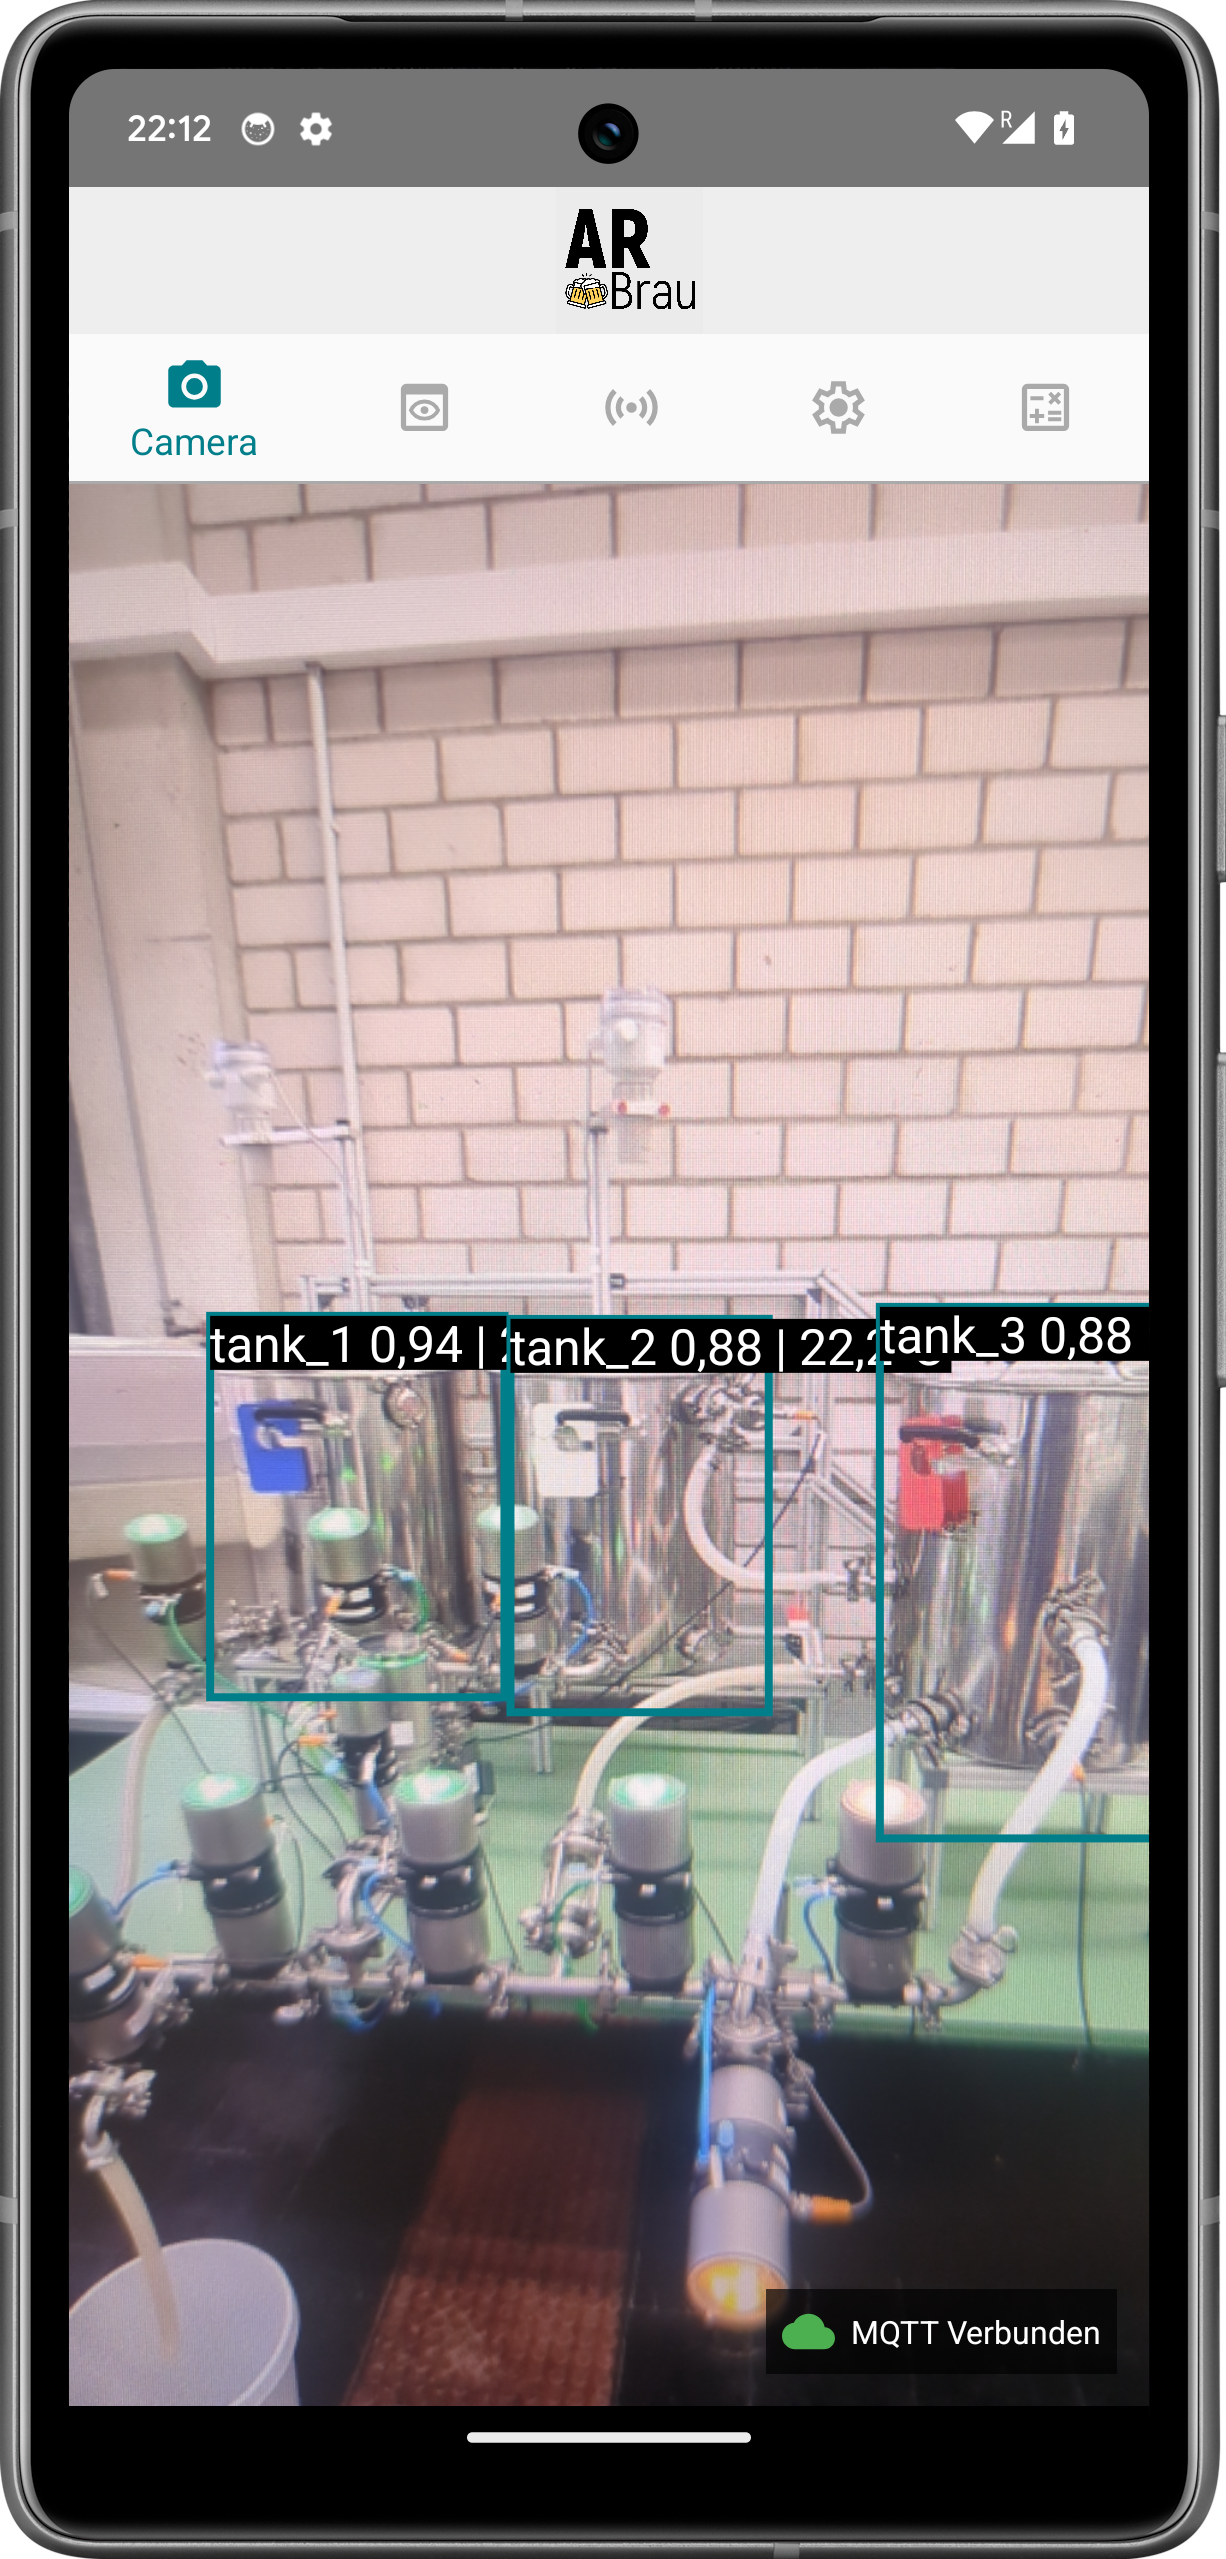
\includegraphics[height=8cm]{pictures/AndroidApp/CameraView.png}
        \caption{Camera}
    \end{subfigure}
    \hfill
    \begin{subfigure}[t]{0.32\textwidth}
        \centering
        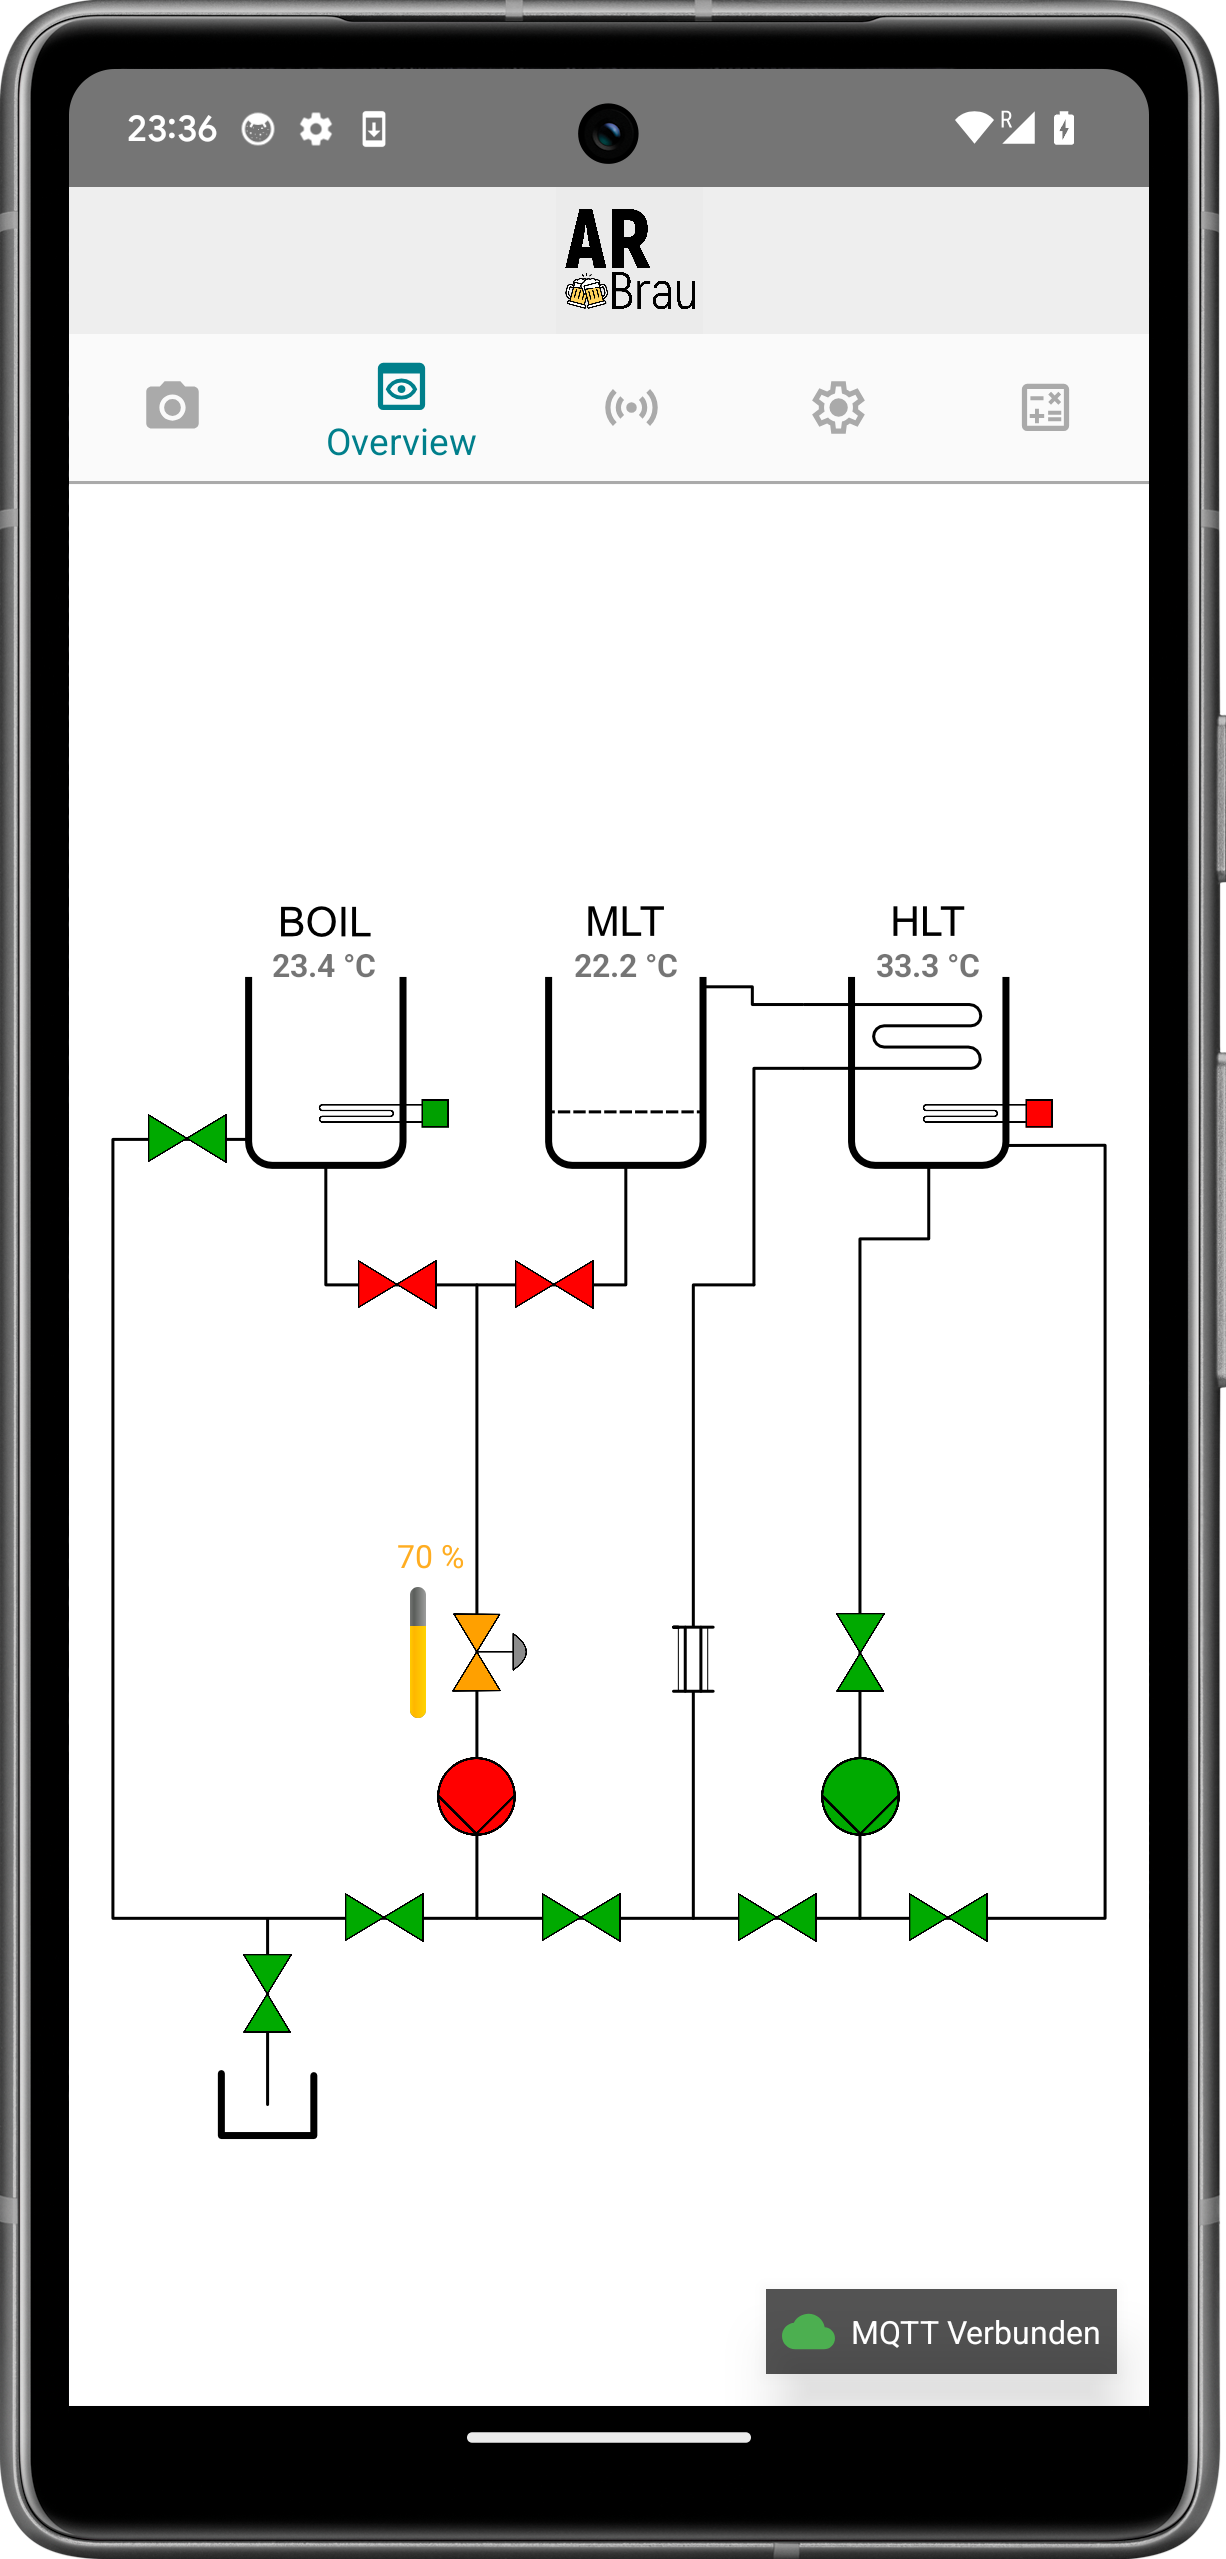
\includegraphics[height=8cm]{pictures/AndroidApp/OverviewTab.png}
        \caption{Overview}
    \end{subfigure}
    \hfill
    \begin{subfigure}[t]{0.32\textwidth}
        \centering
        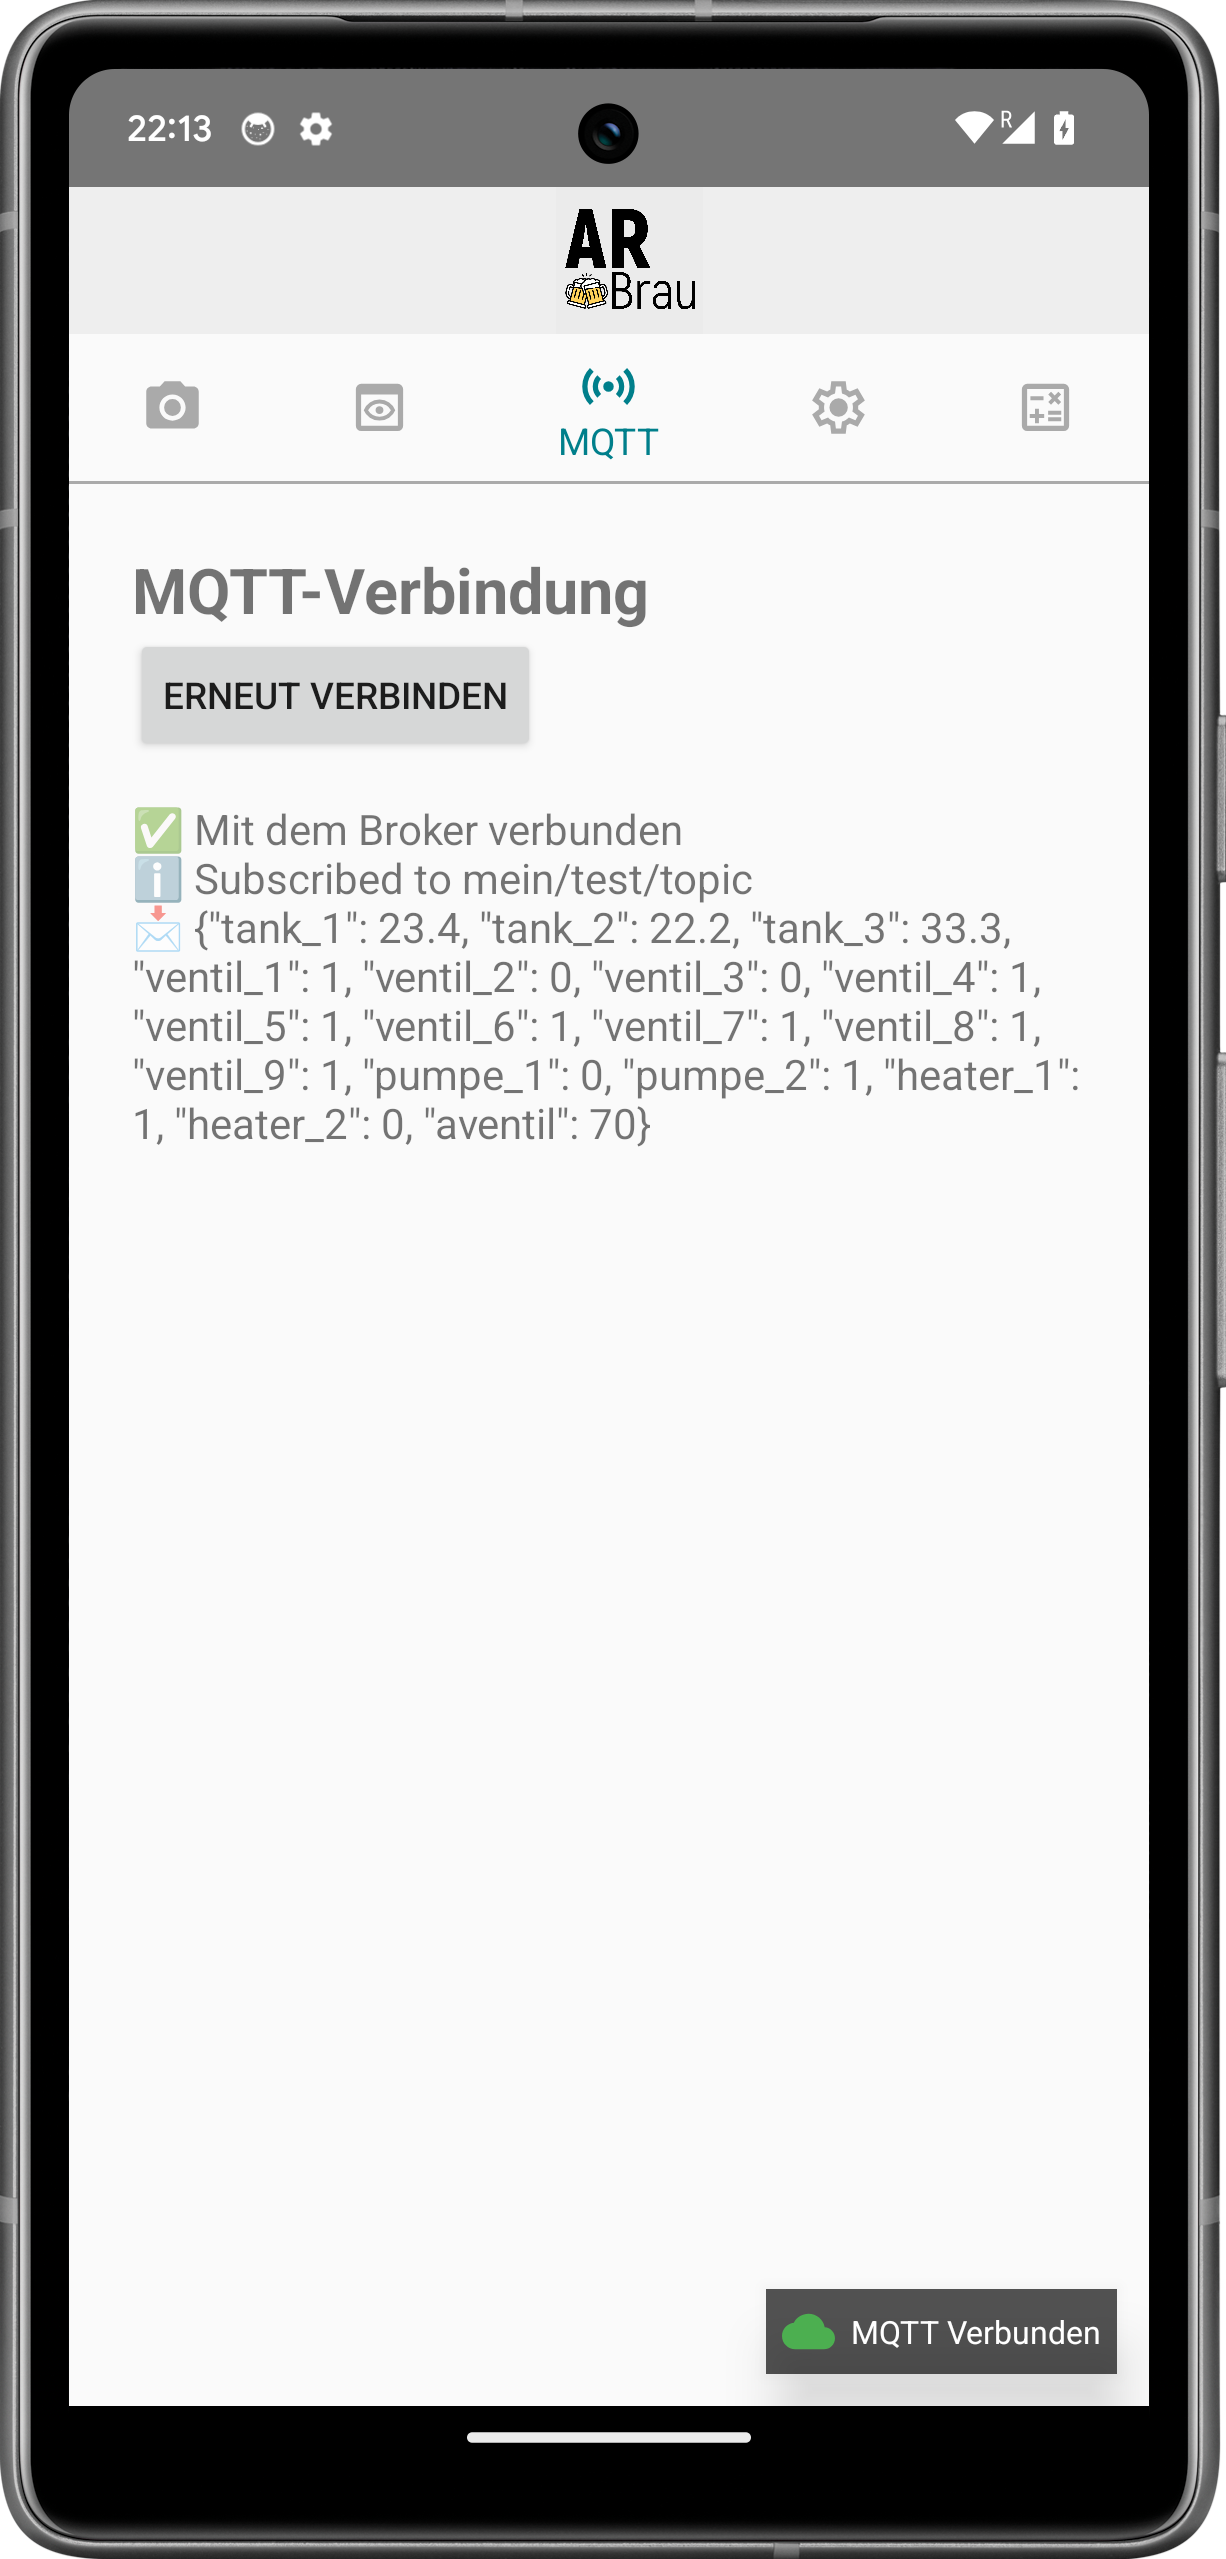
\includegraphics[height=8cm]{pictures/AndroidApp/MQTT.png}
        \caption{MQTT}
    \end{subfigure}

    \vspace{0.5cm} % Abstand zwischen den Reihen

    % --- Zweite Reihe ---
    \begin{subfigure}[t]{0.32\textwidth}
        \centering
        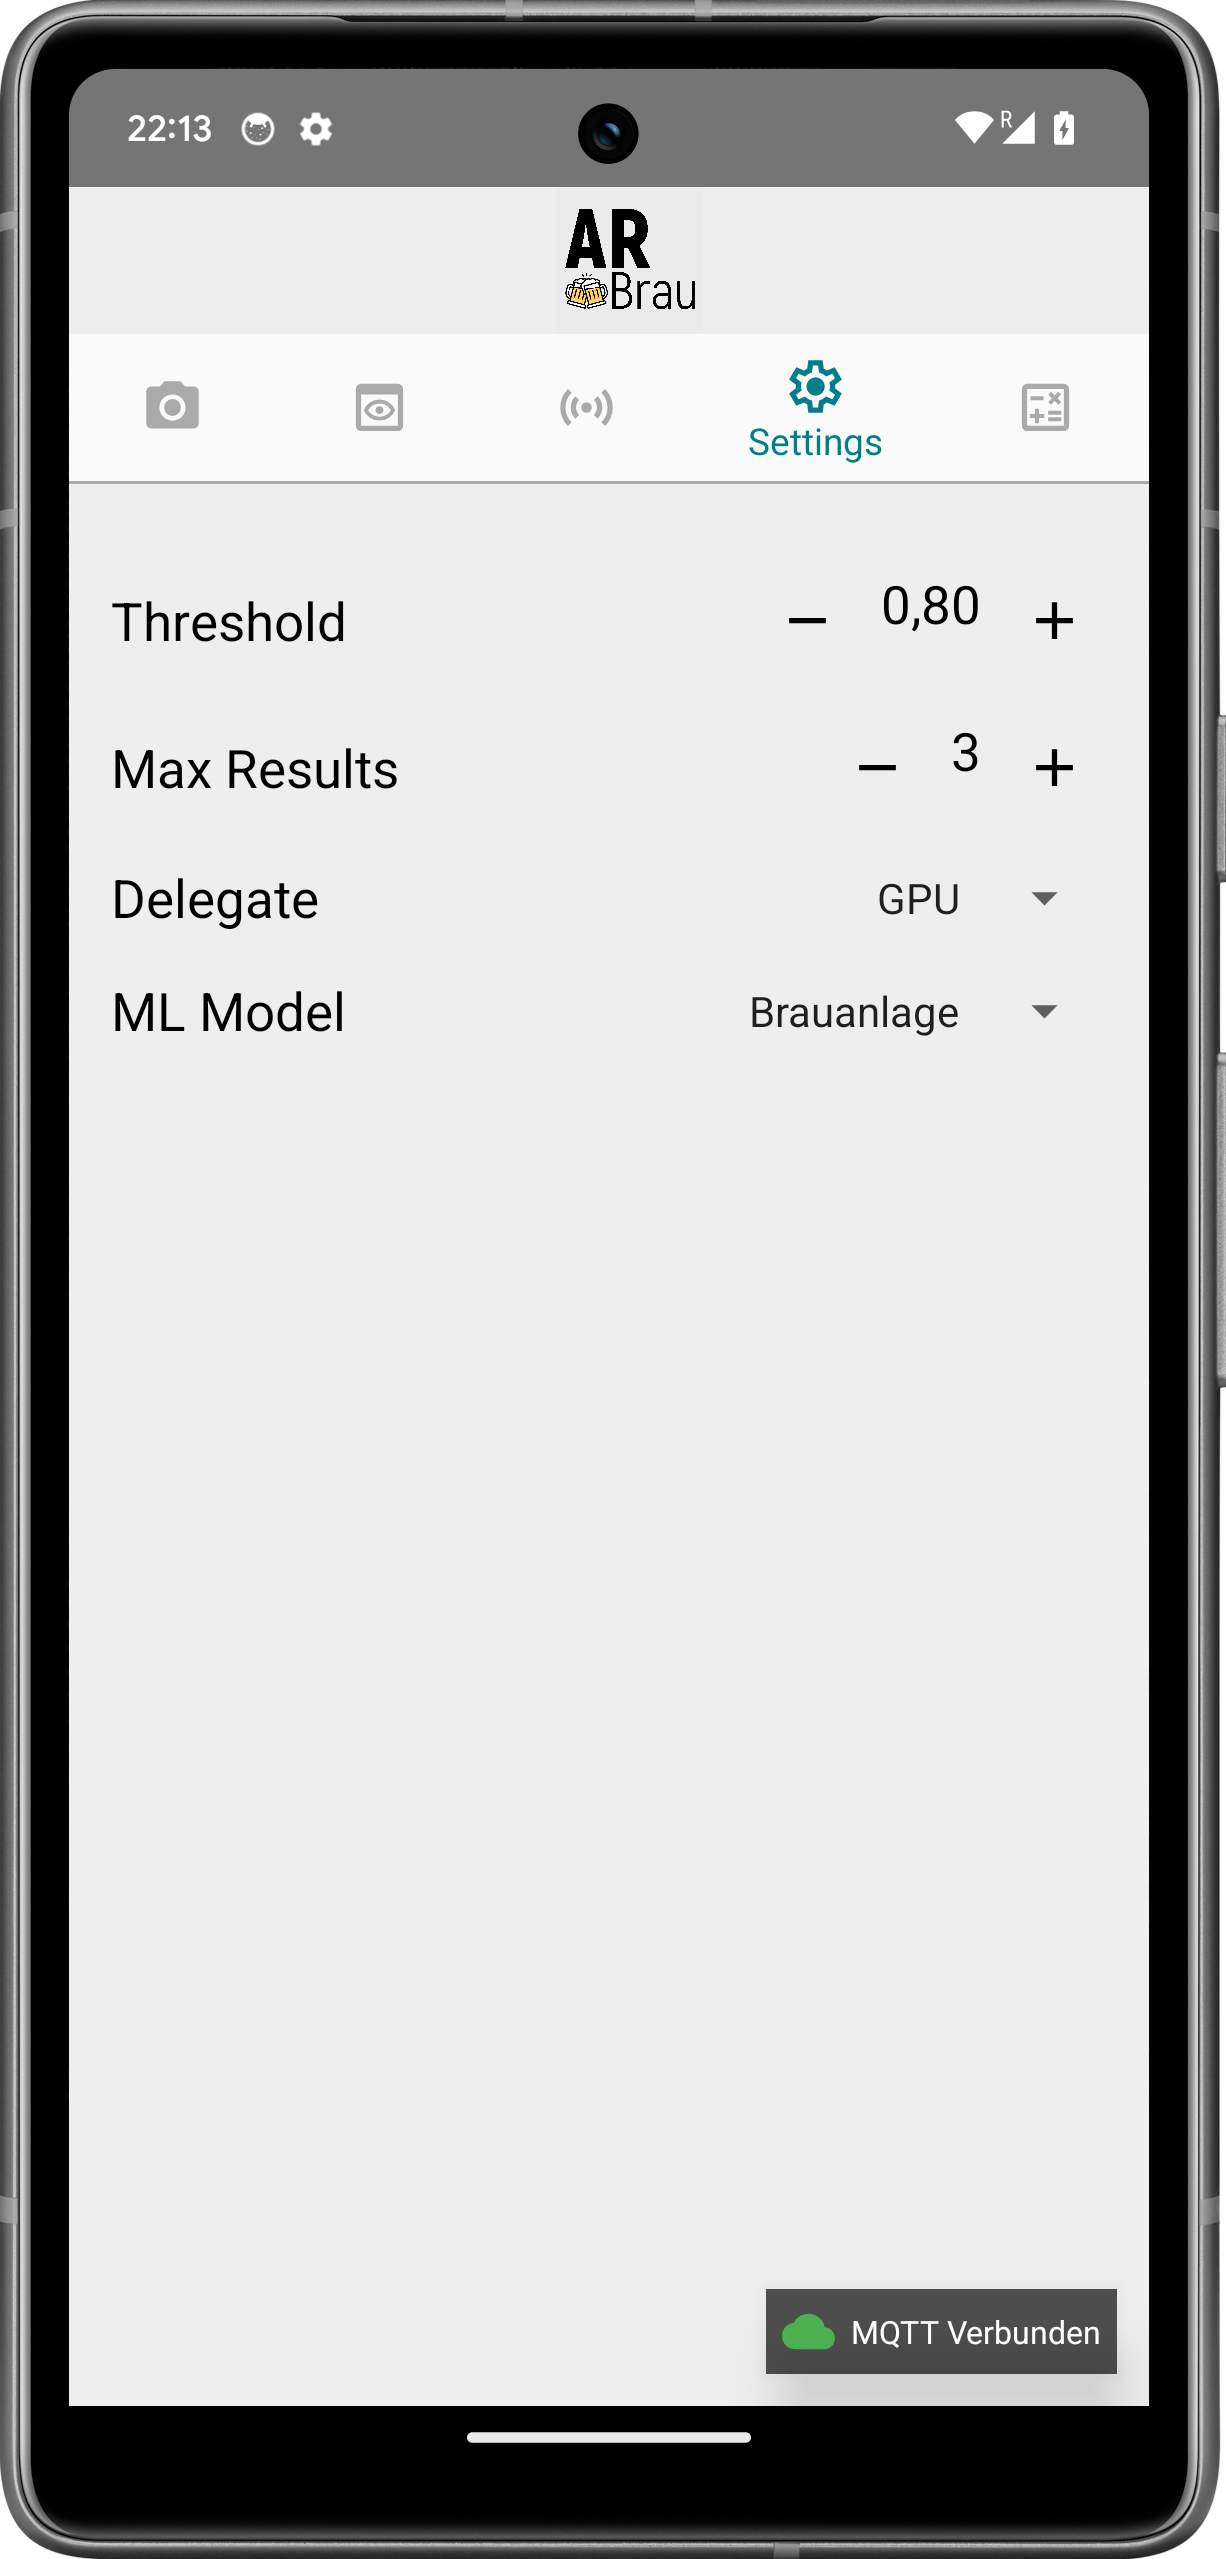
\includegraphics[height=8cm]{pictures/AndroidApp/Settings.png}
        \caption{Settings}
    \end{subfigure}
    \begin{subfigure}[t]{0.32\textwidth}
        \centering
        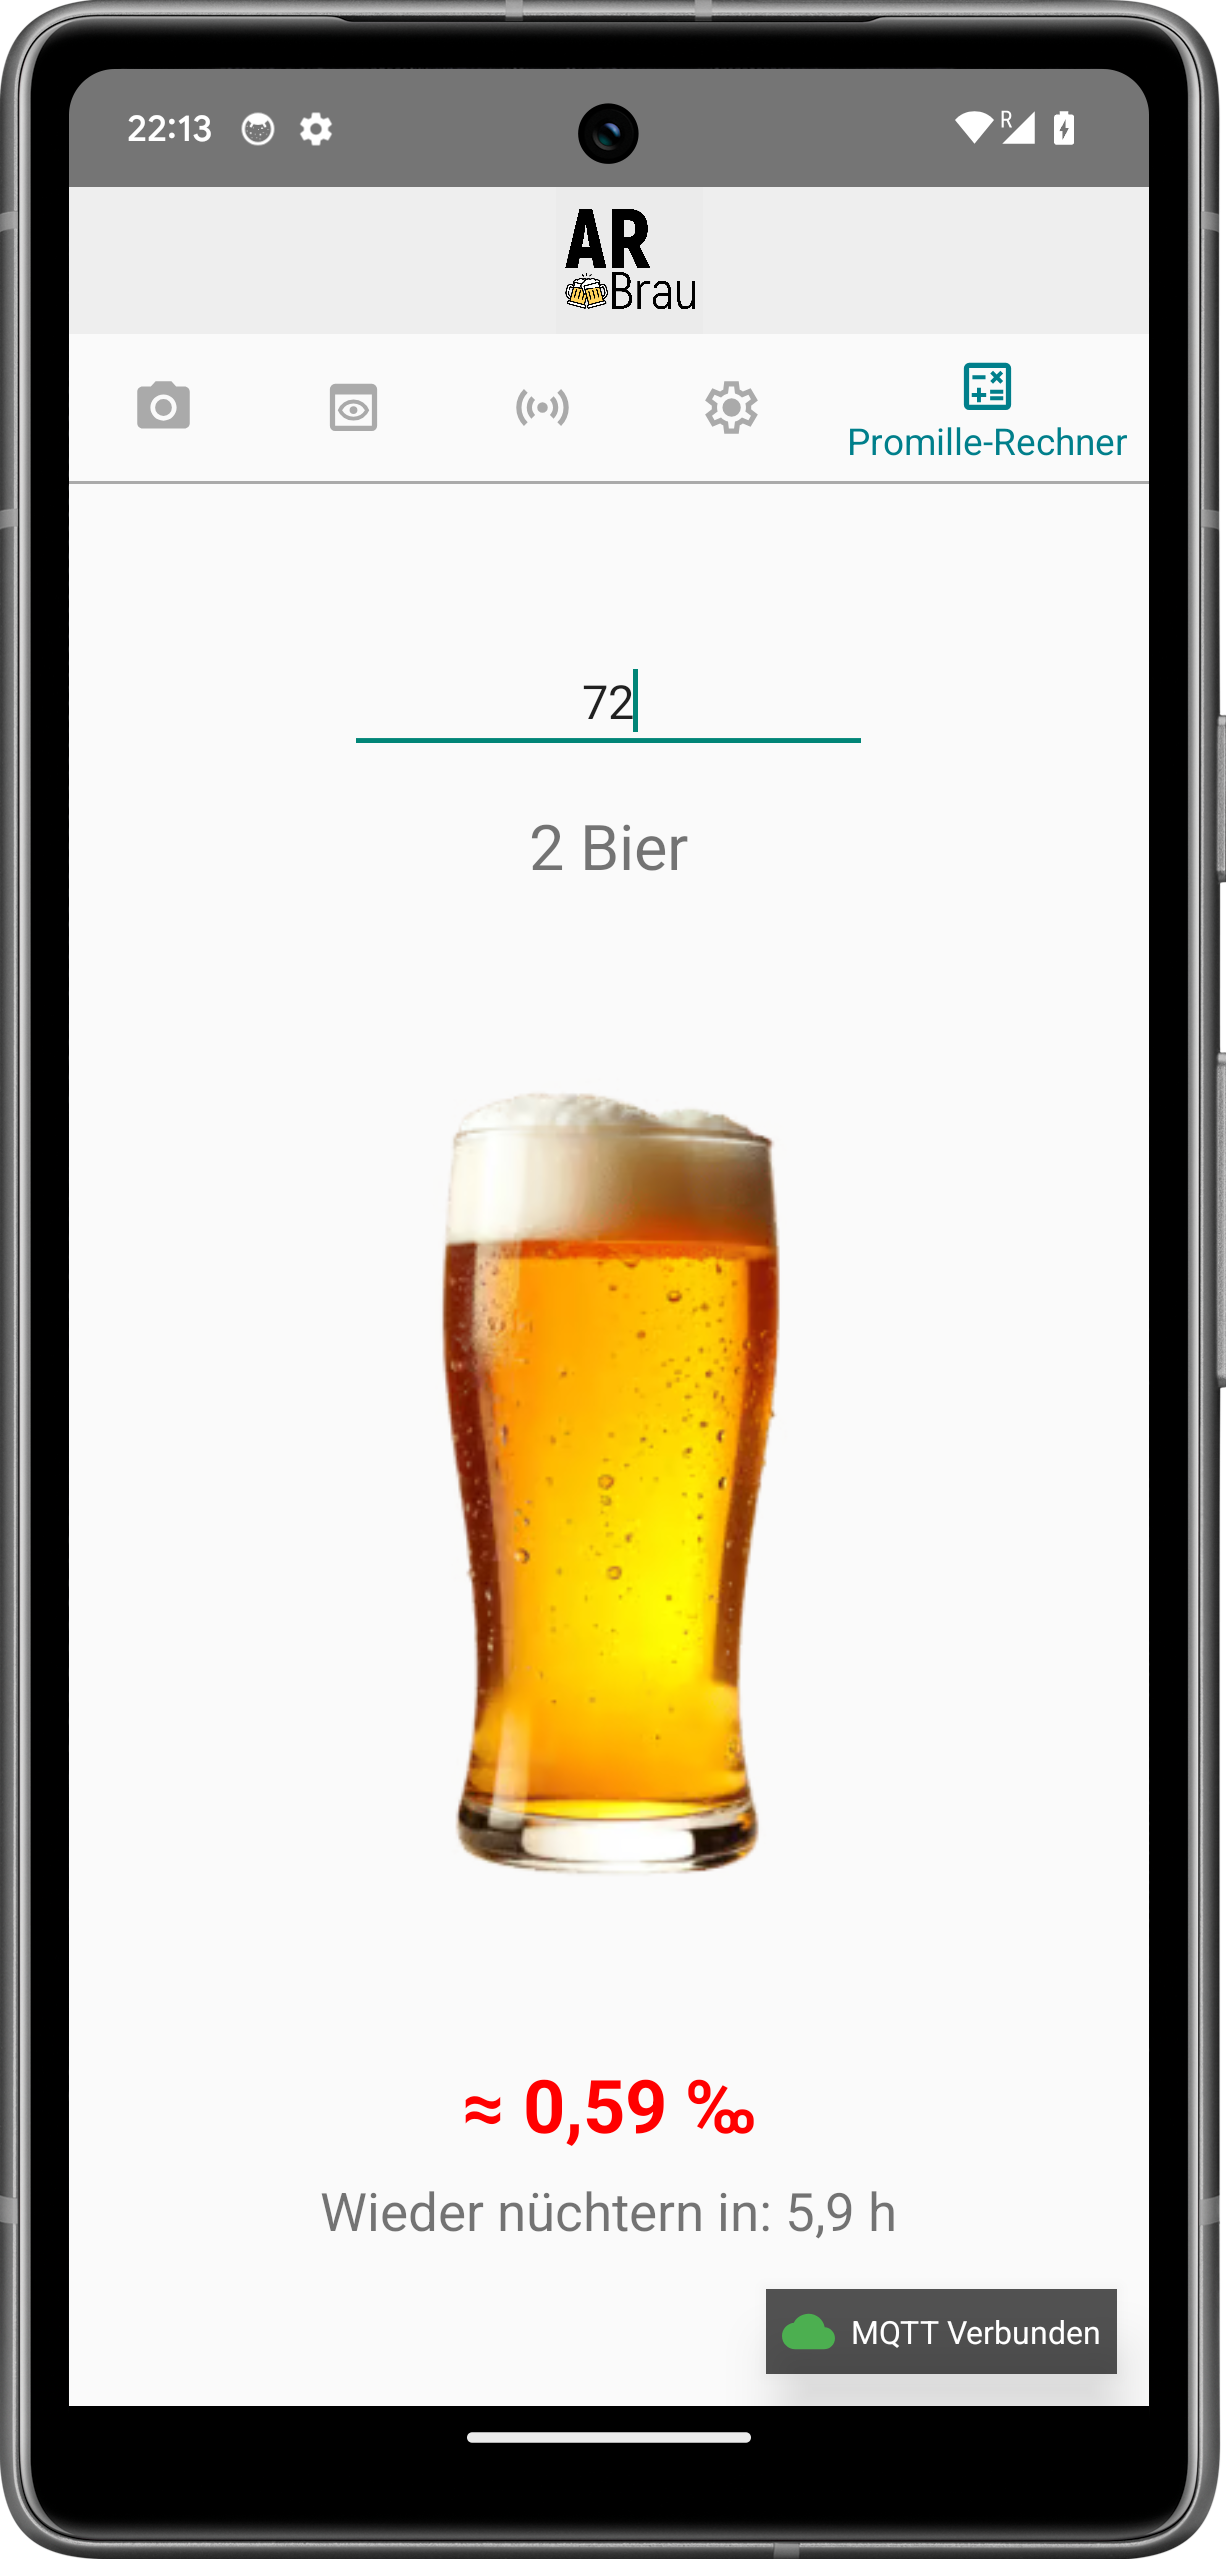
\includegraphics[height=8cm]{pictures/AndroidApp/PromilleRechner.png}
        \caption{Promille Rechner}
    \end{subfigure}

    \caption{Die verschiedenen Tabs der Android App \cite{AppTabs}}
    \label{fig:AppTabs}
\end{figure}

Die verschiedenen Tabs der Android App sind in Abbildung \ref{fig:AppTabs} zu sehen.




Die verwendete Nummerierung der Aktoren/Sensoren in der Android App ist in Abbildung \ref{fig:NummerierungAktorenSensoren} zu sehen. 
\begin{figure}[h!]
    \centering
    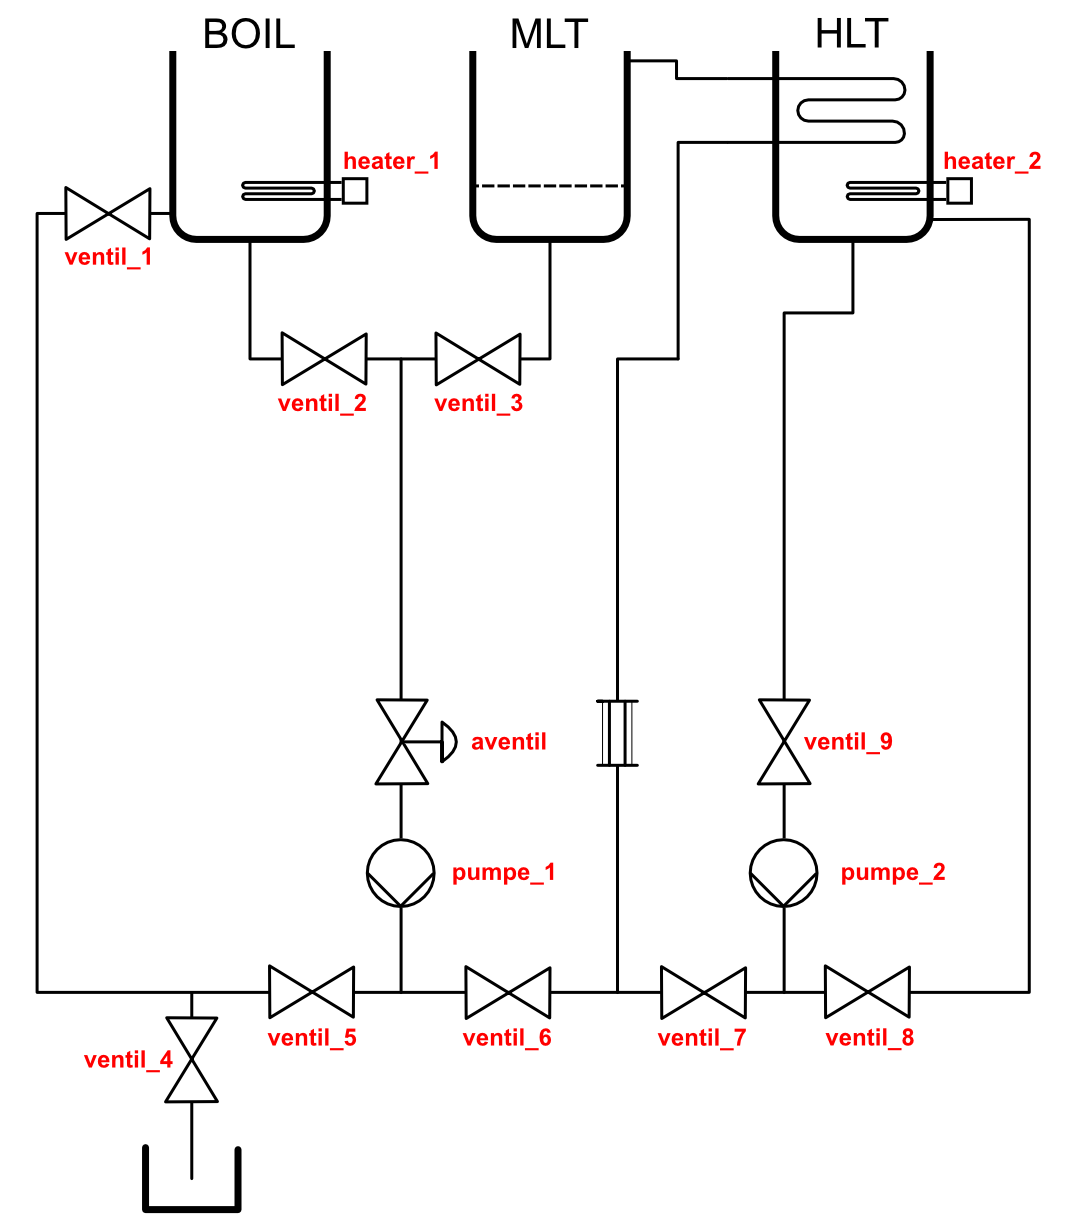
\includegraphics[height=8cm]{pictures/AndroidApp/Nummerierung.png}
    \caption{Nummerierung der Aktoren/Sensoren} \cite{NummerierungAktorenSensoren}
    \label{fig:NummerierungAktorenSensoren}
\end{figure}
